\heading{量子场论-zhx-23秋-期末}

\begin{question}[10 分]
在四维时空化简
\[
\gamma^\mu\gamma_\mu,\qquad
\gamma^\mu\not{k}\gamma_\mu,\qquad
\gamma^\mu\not{k}\not{p}\gamma_\mu.
\]
\begin{solution}
采用
\[
\{\gamma^\mu,\gamma^\nu\}=2g^{\mu\nu},\qquad g^\mu{}_{\mu}=4.
\]
第一式直接为
\[
\boxed{\gamma^\mu\gamma_\mu=4}.
\]
对第二式，先用
\[
\gamma^\mu\gamma^\alpha\gamma_\mu
=2\gamma^\alpha-\gamma^\alpha\gamma^\mu\gamma_\mu
=(2-4)\gamma^\alpha=-2\gamma^\alpha,
\]
故
\[
\boxed{\gamma^\mu\not{k}\gamma_\mu=-2\not{k}}.
\]
对第三式，
\[
\begin{aligned}
\gamma^\mu\gamma^\alpha\gamma^\beta\gamma_\mu
&=(2g^{\mu\alpha}-\gamma^\alpha\gamma^\mu)\gamma^\beta\gamma_\mu\\
&=2\gamma^\beta\gamma^\alpha-
\gamma^\alpha(2\gamma^\beta-\gamma^\beta\gamma^\mu\gamma_\mu)\\
&=2(\gamma^\beta\gamma^\alpha+\gamma^\alpha\gamma^\beta)
=4g^{\alpha\beta}.
\end{aligned}
\]
因此
\[
\boxed{\gamma^\mu\not{k}\not{p}\gamma_\mu=4\,k\cdot p}.
\]
\end{solution}
\end{question}

\begin{question}[20 分]
给定自由费米子拉氏量
\[
\mathcal L=\ii\bar\psi\gamma^\mu\partial_\mu\psi-m\bar\psi\psi.
\]
\begin{enumerate}
  \item 求 $\psi$ 所满足的运动方程；
  \item 证明 $\psi$ 同时满足 Klein--Gordon 方程。
\end{enumerate}
\begin{solution}
\begin{enumerate}
  \item 把 $\psi$ 与 $\bar\psi$ 视为独立场，对 $\bar\psi$ 作 Euler--Lagrange 变分，得到
  \[
  \boxed{(\ii\gamma^\mu\partial_\mu-m)\psi=0}.
  \]

  \item 从左乘以 $(\ii\gamma^\nu\partial_\nu+m)$：
  \[
  (\ii\gamma^\nu\partial_\nu+m)(\ii\gamma^\mu\partial_\mu-m)\psi=0.
  \]
  交叉项相消，并且
  \[
  \gamma^\nu\gamma^\mu\partial_\nu\partial_\mu
  =\frac12\{\gamma^\nu,\gamma^\mu\}\partial_\nu\partial_\mu
  =g^{\nu\mu}\partial_\nu\partial_\mu=\Box,
  \]
  因为 $\partial_\nu\partial_\mu$ 对指标对称，反对易子的反对称部分不贡献。于是
  \[
  -(\Box+m^2)\psi=0,
  \]
  即
  \[
  \boxed{(\Box+m^2)\psi=0}.
  \]
\end{enumerate}
\end{solution}
\end{question}

\begin{question}[25 分]
给定自由复标量场拉氏量
\[
\mathcal L=\partial^\mu\Phi\,\partial_\mu\Phi^*-m^2\Phi\Phi^*.
\]
\begin{enumerate}
  \item 写下 $\Phi$ 和 $\Phi^*$ 的产生湮灭算符展开；
  \item 写下 $\Phi$ 和 $\Phi^*$ 应满足的等时对易关系，并写下产生湮灭算符的所有对易关系；
  \item 写下该拉氏量所具有的整体内部对称性及相应守恒流；
  \item 求复标量场的运动方程，并用其验证上一小题的流守恒；
  \item 将守恒流时间分量的全空间积分用产生湮灭算符表示，并说明其意义。
\end{enumerate}
\begin{solution}
记 $E_{\mathbf p}=\sqrt{\mathbf p^2+m^2}$，采用 Lorentz 不变归一化。
\begin{enumerate}
  \item
  \[
  \boxed{
  \Phi(x)=\int\frac{\dd[3]{p}}{(2\pi)^3\,2E_{\mathbf p}}
  \left[a_{\mathbf p}\ee^{-\ii p\cdot x}+b_{\mathbf p}^\dagger\ee^{\ii p\cdot x}\right]},
  \]
  \[
  \boxed{
  \Phi^*(x)=\int\frac{\dd[3]{p}}{(2\pi)^3\,2E_{\mathbf p}}
  \left[a_{\mathbf p}^\dagger\ee^{\ii p\cdot x}+b_{\mathbf p}\ee^{-\ii p\cdot x}\right]}.
  \]

  \item 共轭动量为
  \[
  \Pi=\partial_0\Phi^*,\qquad \Pi^*=\partial_0\Phi.
  \]
  等时正则对易关系为
  \[
  [\Phi(t,\mathbf x),\Pi(t,\mathbf y)]=\ii\delta^{(3)}(\mathbf x-\mathbf y),
  \]
  \[
  [\Phi^*(t,\mathbf x),\Pi^*(t,\mathbf y)]=\ii\delta^{(3)}(\mathbf x-\mathbf y),
  \]
  其余场--场、动量--动量以及交叉对易子均为零。由此得到
  \[
  \boxed{[a_{\mathbf p},a_{\mathbf q}^\dagger]
  =(2\pi)^3 2E_{\mathbf p}\delta^{(3)}(\mathbf p-\mathbf q)},
  \]
  \[
  \boxed{[b_{\mathbf p},b_{\mathbf q}^\dagger]
  =(2\pi)^3 2E_{\mathbf p}\delta^{(3)}(\mathbf p-\mathbf q)},
  \]
  以及
  \[
  [a,a]=[a^\dagger,a^\dagger]=[b,b]=[b^\dagger,b^\dagger]
  =[a,b]=[a,b^\dagger]=[a^\dagger,b]=[a^\dagger,b^\dagger]=0.
  \]

  \item 取整体 $U(1)$ 变换
  \[
  \Phi\to\ee^{-\ii\alpha}\Phi,
  \qquad
  \Phi^*\to\ee^{\ii\alpha}\Phi^*,
  \]
  则 Noether 流可取
  \[
  \boxed{j^\mu=\ii\left(\Phi^*\partial^\mu\Phi-\Phi\partial^\mu\Phi^*\right)}.
  \]

  \item Euler--Lagrange 方程为
  \[
  \boxed{(\Box+m^2)\Phi=0},\qquad
  \boxed{(\Box+m^2)\Phi^*=0}.
  \]
  因此
  \[
  \begin{aligned}
  \partial_\mu j^\mu
  &=\ii\left(\Phi^*\Box\Phi-\Phi\Box\Phi^*\right)\\
  &=\ii\left[-m^2\Phi^*\Phi+m^2\Phi\Phi^*\right]=0.
  \end{aligned}
  \]

  \item 正常序后的守恒荷为
  \[
  \boxed{
  Q=\int\frac{\dd[3]{p}}{(2\pi)^3\,2E_{\mathbf p}}
  \left(a_{\mathbf p}^\dagger a_{\mathbf p}
  -b_{\mathbf p}^\dagger b_{\mathbf p}\right)}.
  \]
  它测量粒子数与反粒子数之差(再乘实际电荷单位即可成为电荷)。若不作正常序，$b b^\dagger$ 会带来与真空有关的无穷常数；正常序把真空荷取为零。
\end{enumerate}
\end{solution}
\end{question}

\begin{question}[30 分]
通过极小耦合引入复标量场与电磁场的相互作用：
\[
\mathcal L=D^\mu\Phi(D_\mu\Phi)^*-m^2\Phi\Phi^*-\frac14F_{\mu\nu}F^{\mu\nu},
\]
其中
\[
D_\mu=\partial_\mu+\ii eA_\mu,
\qquad
F_{\mu\nu}=\partial_\mu A_\nu-\partial_\nu A_\mu.
\]
\begin{enumerate}
  \item 写下定域规范对称性及对应场变换；
  \item 写下动量空间费曼规则，包括传播子、相互作用顶点和外线极化因子；
  \item 树图水平计算 $\Phi(p_1)+\Phi^*(p_2)\to\gamma(k_1)+\gamma(k_2)$ 的散射振幅 $\mathcal M$；
  \item 将振幅写成 $\mathcal M=M_\mu\epsilon^{\mu,*}(k_1)$，具体计算 $M_\mu k_1^\mu$；
  \item 单圈水平画出 $\gamma(p_1)+\gamma(p_2)\to\gamma(k_1)+\gamma(k_2)$ 的所有费曼图并写下振幅，无需求积分；
  \item 计算上一小问振幅的发散项系数。
\end{enumerate}
\begin{solution}
\begin{enumerate}
  \item 与题目 $D_\mu=\partial_\mu+\ii eA_\mu$ 的号数一致，可取
  \[
  \boxed{\Phi'(x)=\ee^{-\ii e\alpha(x)}\Phi(x)},\qquad
  \boxed{A_\mu'(x)=A_\mu(x)+\partial_\mu\alpha(x)}.
  \]
  于是 $D_\mu'\Phi'=\ee^{-\ii e\alpha}D_\mu\Phi$，而 $F_{\mu\nu}$ 不变。

  \item 在 Feynman 规范下：
  \[
  \text{标量传播子:}\qquad \frac{\ii}{p^2-m^2+\ii0},
  \]
  \[
  \text{光子传播子:}\qquad \frac{-\ii g_{\mu\nu}}{k^2+\ii0}.
  \]
  三点顶点(标量线上入、出动量分别为 $p,p'$)可写为
  \[
  \boxed{\ii e(p+p')^\mu},
  \]
  四点 seagull 顶点为
  \[
  \boxed{2\ii e^2g^{\mu\nu}}.
  \]
  外线实光子带 $\epsilon^\mu(k)$；出射光子用 $\epsilon^{\mu,*}(k)$。

  \item 树图有两个标量交换图和一个 seagull 接触图。图中实线箭头表示带电标量，虚线表示光子：
  \begin{center}
  \begin{tikzpicture}[scale=0.84,line cap=round]
    \begin{scope}[xshift=-4.5cm]
      \fill (-0.45,0) circle (2pt); \fill (0.45,0) circle (2pt);
      \draw[thick,->] (-1.65,-0.8)--(-0.5,-0.05); \draw[thick,->] (1.65,-0.8)--(0.5,-0.05);
      \draw[thick,->] (-0.45,0)--(0.45,0);
      \draw[thick,dashed] (-0.45,0)--(-1.55,0.85); \draw[thick,dashed] (0.45,0)--(1.55,0.85);
      \node[font=\scriptsize] at (0,-1.2) {$t$ 通道};
    \end{scope}
    \begin{scope}
      \fill (-0.45,0) circle (2pt); \fill (0.45,0) circle (2pt);
      \draw[thick,->] (-1.65,-0.8)--(-0.5,-0.05); \draw[thick,->] (1.65,-0.8)--(0.5,-0.05);
      \draw[thick,->] (-0.45,0)--(0.45,0);
      \draw[thick,dashed] (-0.45,0)--(1.55,0.85); \draw[thick,dashed] (0.45,0)--(-1.55,0.85);
      \node[font=\scriptsize] at (0,-1.2) {$u$ 通道};
    \end{scope}
    \begin{scope}[xshift=4.5cm]
      \fill (0,0) circle (2.4pt);
      \draw[thick,->] (-1.55,-0.8)--(-0.08,-0.04); \draw[thick,->] (1.55,-0.8)--(0.08,-0.04);
      \draw[thick,dashed] (0,0)--(-1.45,0.85); \draw[thick,dashed] (0,0)--(1.45,0.85);
      \node[font=\scriptsize] at (0,-1.2) {seagull};
    \end{scope}
  \end{tikzpicture}
  \end{center}
  取
  \[
  D_t=(p_1-k_1)^2-m^2,\qquad
  D_u=(p_1-k_2)^2-m^2,
  \]
  并用 $p_1+p_2=k_1+k_2$。可写
  \[
  \boxed{
  \mathcal M=e^2\epsilon_\mu^*(k_1)\epsilon_\nu^*(k_2)
  \left[
  2g^{\mu\nu}
  +\frac{(2p_1-k_1)^\mu(2p_2-k_2)^\nu}{D_t}
  +\frac{(2p_2-k_1)^\mu(2p_1-k_2)^\nu}{D_u}
  \right]}.
  \]
  这里整体相位取决于 $S$ 矩阵与顶点的约定，但三项的相对号由规范不变性固定。

  \item 去掉第一只光子的极化向量，定义
  \[
  M^\mu=e^2\epsilon_\nu^*(k_2)\left[
  2g^{\mu\nu}
  +\frac{(2p_1-k_1)^\mu(2p_2-k_2)^\nu}{D_t}
  +\frac{(2p_2-k_1)^\mu(2p_1-k_2)^\nu}{D_u}
  \right].
  \]
  对实光子 $k_1^2=0$ 且外标量满足 $p_i^2=m^2$，故
  \[
  D_t=-2p_1\cdot k_1,
  \qquad
  D_u=-2p_2\cdot k_1.
  \]
  从而
  \[
  \frac{k_1\cdot(2p_1-k_1)}{D_t}=-1,
  \qquad
  \frac{k_1\cdot(2p_2-k_1)}{D_u}=-1.
  \]
  因此
  \[
  \begin{aligned}
  k_{1\mu}M^\mu/e^2
  &=\epsilon_\nu^*(k_2)
  \left[2k_1^\nu-(2p_2-k_2)^\nu-(2p_1-k_2)^\nu\right]\\
  &=2\epsilon_\nu^*(k_2)
  [k_1-(p_1+p_2-k_2)]^\nu=0.
  \end{aligned}
  \]
  故
  \[
  \boxed{k_{1\mu}M^\mu=0},
  \]
  即满足 Ward 恒等式。

  \item 一圈四光子振幅有三类拓扑：四个三点顶点的 box 图；一个 seagull 与两个三点顶点的 triangle 图；两个 seagull 的 bubble 图。代表性图如下。虚线为外光子，闭合实线为带电标量环；对外线 $1,2,3,4$ 的允许置换分别给出 $3$ 个 box、$6$ 个 triangle 与 $3$ 个 bubble。
  \begin{center}
  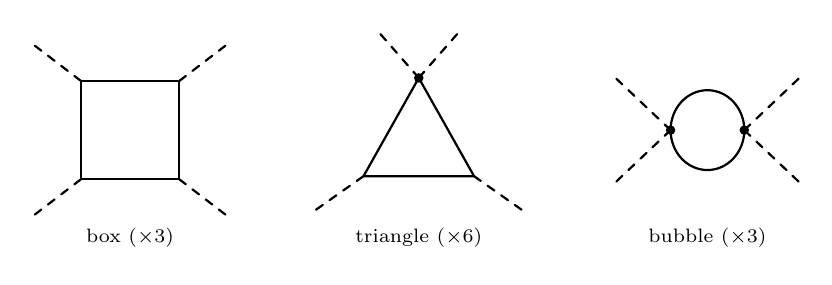
\begin{tikzpicture}[scale=0.78,line cap=round,line join=round]
    % box
    \begin{scope}[xshift=-4.7cm]
      \draw[thick] (-0.8,-0.8)--(0.8,-0.8)--(0.8,0.8)--(-0.8,0.8)--cycle;
      \foreach \x/\y/\xx/\yy in {-0.8/0.8/-1.65/1.45,0.8/0.8/1.65/1.45,-0.8/-0.8/-1.65/-1.45,0.8/-0.8/1.65/-1.45}{\draw[thick,dashed] (\x,\y)--(\xx,\yy);}
      \node[font=\scriptsize] at (0,-1.75) {box ($\times3$)};
    \end{scope}
    % triangle
    \begin{scope}
      \coordinate (a) at (-0.9,-0.75); \coordinate (b) at (0.9,-0.75); \coordinate (c) at (0,0.85);
      \draw[thick] (a)--(b)--(c)--cycle;
      \draw[thick,dashed] (a)--(-1.75,-1.35); \draw[thick,dashed] (b)--(1.75,-1.35);
      \draw[thick,dashed] (c)--(-0.7,1.65); \draw[thick,dashed] (c)--(0.7,1.65);
      \fill (c) circle (2.2pt);
      \node[font=\scriptsize] at (0,-1.75) {triangle ($\times6$)};
    \end{scope}
    % bubble
    \begin{scope}[xshift=4.7cm]
      \fill (-0.6,0) circle (2.2pt); \fill (0.6,0) circle (2.2pt);
      \draw[thick] (-0.6,0) arc (180:0:0.6 and 0.65); \draw[thick] (0.6,0) arc (0:-180:0.6 and 0.65);
      \draw[thick,dashed] (-0.6,0)--(-1.55,0.9); \draw[thick,dashed] (-0.6,0)--(-1.55,-0.9);
      \draw[thick,dashed] (0.6,0)--(1.55,0.9); \draw[thick,dashed] (0.6,0)--(1.55,-0.9);
      \node[font=\scriptsize] at (0,-1.75) {bubble ($\times3$)};
    \end{scope}
  \end{tikzpicture}
  \end{center}

  可将总振幅写成
  \[
  \boxed{\mathcal M^{\mu\nu\rho\sigma}_{1\text{-loop}}
  =\sum_{\rm box}\mathcal M_{\rm box}^{\mu\nu\rho\sigma}
  +\sum_{\rm tri}\mathcal M_{\rm tri}^{\mu\nu\rho\sigma}
  +\sum_{\rm bub}\mathcal M_{\rm bub}^{\mu\nu\rho\sigma}}.
  \]
  例如给定环上排序 $(1,2,3,4)$，box 项的被积函数可写为
  \[
  \mathcal M_{\rm box}^{\mu_1\mu_2\mu_3\mu_4}
  =e^4\int\frac{\dd[d]{\ell}}{(2\pi)^d}
  \frac{N^{\mu_1\mu_2\mu_3\mu_4}(\ell)}
  {D_0D_1D_2D_3},
  \]
  其中
  \[
  D_j=q_j^2-m^2+\ii0,
  \qquad q_0=\ell,\quad q_j=\ell+k_1+\cdots+k_j,
  \]
  而 $N$ 是四个标量--光子顶点因子 $(q_i+q_{i+1})^{\mu}$ 的乘积。triangle 项把其中一对相邻光子替换为 $2e^2g^{\mu\nu}$ 的 seagull 顶点，bubble 项则含两个这样的张量。对所有外线排列求和即可得到完整振幅。

  \item 为避免只凭“规范不变性”判断，直接抽取各拓扑的 UV 极点。UV 发散是局域的，因此可在保持标量质量 $m\neq0$ 以避免红外问题的同时，把外动量在极点系数中置零。记
  \[
  T^{\mu\nu\rho\sigma}=g^{\mu\nu}g^{\rho\sigma}
  +g^{\mu\rho}g^{\nu\sigma}+g^{\mu\sigma}g^{\nu\rho}.
  \]
  在 $D=4-2\epsilon$ 中需要的极点为
  \[
  \int\frac{\dd[D]{\ell}}{(2\pi)^D}
  \frac{\ell^\mu\ell^\nu\ell^\rho\ell^\sigma}{(\ell^2-m^2)^4}
  \Big|_{\rm div}
  =\frac{\ii}{16\pi^2\epsilon}\frac1{24}
  T^{\mu\nu\rho\sigma},
  \]
  \[
  \int\frac{\dd[D]{\ell}}{(2\pi)^D}
  \frac{\ell^\rho\ell^\sigma}{(\ell^2-m^2)^3}
  \Big|_{\rm div}
  =\frac{\ii}{16\pi^2\epsilon}\frac14g^{\rho\sigma},
  \qquad
  \int\frac{\dd[D]{\ell}}{(2\pi)^D}
  \frac1{(\ell^2-m^2)^2}
  \Big|_{\rm div}
  =\frac{\ii}{16\pi^2\epsilon}.
  \]
  box 图的每个三点顶点在大环动量下给出 $2e\ell^\mu$。三个不等价环排序相加得到
  \[
  \ii\Gamma_{\rm box,div}^{\mu\nu\rho\sigma}
  =\frac{\ii e^4}{8\pi^2\epsilon}T^{\mu\nu\rho\sigma}.
  \]
  triangle 图含一个 $2\ii e^2g^{\mu\nu}$ seagull 顶点和两个三点顶点。六个外线分配中，每一种指标配对出现两次，因此
  \[
  \ii\Gamma_{\rm tri,div}^{\mu\nu\rho\sigma}
  =-\frac{\ii e^4}{4\pi^2\epsilon}T^{\mu\nu\rho\sigma}.
  \]
  bubble 图含两个 seagull 顶点；两个相同内部标量线带来对称因子 $1/2$。三个外线配对相加给出
  \[
  \ii\Gamma_{\rm bub,div}^{\mu\nu\rho\sigma}
  =\frac{\ii e^4}{8\pi^2\epsilon}T^{\mu\nu\rho\sigma}.
  \]
  因而极点逐项相消：
  \[
  \ii\Gamma_{\rm div}
  =\frac{\ii e^4}{8\pi^2\epsilon}(1-2+1)
  T^{\mu\nu\rho\sigma}=0.
  \]
  所以
  \[
  \boxed{\mathcal M^{(1)}_{\gamma\gamma\to\gamma\gamma,\,\mathrm{div}}=0}.
  \]
  这与 Ward 恒等式及“标量 QED 中不存在独立的规范不变 $A^4$ 维数四反项”相互校验，而不是以该论断代替计算。
\end{enumerate}
\end{solution}
\end{question}

\begin{question}[15 分]
考虑定义在五维时空的 $U(1)$ 规范理论
\[
S=\int\dd[5]{x}\left[-\frac14F_{MN}F^{MN}\right],
\]
其中
\[
x^M=(x^\mu,x^5),\quad M=0,1,2,3,5,\quad \mu=0,1,2,3,
\]
\[
F_{MN}=\partial_MA_N-\partial_NA_M,
\qquad
A_M\to A_M+\partial_M\alpha.
\]
将第五维紧致化到半径为 $R$ 的圆：
\[
x^5=R\phi,\qquad \phi\in[0,2\pi],
\]
并展开
\[
A_M(x^\mu,\phi)=A_M^{(0)}(x^\mu)
+\sum_{n=1}^\infty\left(A_M^{(n)}(x^\mu)\ee^{\ii n\phi}+\mathrm{h.c.}\right).
\]
\begin{enumerate}
  \item 证明对非零 $n$ 可通过规范变换令 $A_5^{(n)}=0$，求相应规范函数，并说明为何 $A_5^{(0)}$ 无法如此去掉；
  \item 当 $R$ 远小于可观测尺度时，积掉第五维，写出四维理论拉氏量并给出粒子谱(质量与自旋)。
\end{enumerate}
\begin{solution}
\begin{enumerate}
  \item 将规范参数同样作 Fourier 展开：
  \[
  \alpha(x,\phi)=\alpha^{(0)}(x)+\sum_{n\ge1}
  \left(\alpha^{(n)}(x)\ee^{\ii n\phi}+\mathrm{h.c.}\right).
  \]
  因为
  \[
  \partial_5=\frac1R\partial_\phi,
  \]
  非零模变换为
  \[
  A_5^{(n)}\to A_5^{(n)}+\frac{\ii n}{R}\alpha^{(n)}.
  \]
  取
  \[
  \boxed{\alpha^{(n)}=\frac{\ii R}{n}A_5^{(n)}}
  \]
  即可令变换后的 $A_5^{(n)}$ 为零。对零模却有
  \[
  \delta A_5^{(0)}=\partial_5\alpha^{(0)}=0,
  \]
  所以周期且单值的普通规范变换不能消去 $A_5^{(0)}$；它是四维中的真实标量零模(更全局地说，与圆周 Wilson loop 有关)。

  \item 对 $x^5$ 积分后有共同因子 $2\pi R$。把各 Fourier 模重标度为正则四维动能后，并采用上面的 $A_5^{(n>0)}=0$ 规范，可写
  \[
  \boxed{
  \begin{aligned}
  \mathcal L_{4D}={}&-\frac14F_{\mu\nu}^{(0)}F^{(0)\mu\nu}
  +\frac12\partial_\mu A_5^{(0)}\partial^\mu A_5^{(0)}\\
  &+\sum_{n=1}^\infty\left[
  -\frac12F_{\mu\nu}^{(n)*}F^{(n)\mu\nu}
  +\frac{n^2}{R^2}A_\mu^{(n)*}A^{(n)\mu}
  \right].
  \end{aligned}}
  \]
  这里 $A_\mu^{(n)}$ 是把 $\pm n$ 两个实 Fourier 模合并得到的复矢量场。其质量
  \[
  \boxed{m_n=\frac{n}{R}},\qquad n\ge1.
  \]
  粒子谱为：
  \begin{itemize}
    \item $A_\mu^{(0)}$：四维无质量自旋 $1$ 光子，两个物理极化；
    \item $A_5^{(0)}$：四维无质量实标量，自旋 $0$；
    \item 每个 $n\ge1$：质量 $n/R$ 的复 massive vector $A_\mu^{(n)}$，每个复场含三个物理极化；对应的 $A_5^{(n)}$ 是被吸收的 Stueckelberg/纵向自由度。
  \end{itemize}
  当探测能标 $E\ll1/R$ 时，所有 $n\ge1$ 的 Kaluza--Klein 模都很重并退耦，低能仅剩无质量光子与标量零模。
\end{enumerate}
\end{solution}
\end{question}

\vspace{0.5em}
\begin{center}\textbf{原卷附：可能有用的公式}\end{center}

\[
\sigma^1=\begin{pmatrix}0&1\\1&0\end{pmatrix},\qquad
\sigma^2=\begin{pmatrix}0&-\ii\\\ii&0\end{pmatrix},\qquad
\sigma^3=\begin{pmatrix}1&0\\0&-1\end{pmatrix}.
\]
\[
\gamma^\mu=\begin{pmatrix}0&\sigma^\mu\\\bar\sigma^\mu&0\end{pmatrix}.
\]
\[
\frac1{A_1A_2\cdots A_n}
=\int_0^1\dd{x_1}\cdots\dd{x_n}\,
\delta\!\left(\sum_i x_i-1\right)
\frac{(n-1)!}{(x_1A_1+\cdots+x_nA_n)^n}.
\]
\[
\int\frac{\dd[d]{\ell}}{(2\pi)^d}\frac1{(\ell^2-\Delta)^n}
=\frac{(-1)^n\ii}{(4\pi)^{d/2}}
\frac{\Gamma(n-d/2)}{\Gamma(n)}
\left(\frac1\Delta\right)^{n-d/2}.
\]
\[
\int\frac{\dd[d]{\ell}}{(2\pi)^d}\frac{\ell^2}{(\ell^2-\Delta)^n}
=\frac{(-1)^{n-1}\ii}{(4\pi)^{d/2}}\frac d2
\frac{\Gamma(n-d/2-1)}{\Gamma(n)}
\left(\frac1\Delta\right)^{n-d/2-1}.
\]
\[
\int\frac{\dd[d]{\ell}}{(2\pi)^d}\frac{\ell^\mu\ell^\nu}{(\ell^2-\Delta)^n}
=\frac{(-1)^{n-1}\ii}{(4\pi)^{d/2}}\frac{g^{\mu\nu}}2
\frac{\Gamma(n-d/2-1)}{\Gamma(n)}
\left(\frac1\Delta\right)^{n-d/2-1}.
\]
\[
\int\frac{\dd[d]{\ell}}{(2\pi)^d}\frac{(\ell^2)^2}{(\ell^2-\Delta)^n}
=\frac{(-1)^n\ii}{(4\pi)^{d/2}}\frac{d(d+2)}4
\frac{\Gamma(n-d/2-2)}{\Gamma(n)}
\left(\frac1\Delta\right)^{n-d/2-2}.
\]
\[
\begin{aligned}
&\int\frac{\dd[d]{\ell}}{(2\pi)^d}
\frac{\ell^\mu\ell^\nu\ell^\rho\ell^\sigma}{(\ell^2-\Delta)^n}\\
&\quad=\frac{(-1)^n\ii}{(4\pi)^{d/2}}
\frac{\Gamma(n-d/2-2)}{\Gamma(n)}
\left(\frac1\Delta\right)^{n-d/2-2}
\frac14\left(g^{\mu\nu}g^{\rho\sigma}+g^{\mu\rho}g^{\nu\sigma}+g^{\mu\sigma}g^{\nu\rho}\right).
\end{aligned}
\]
\[
\Gamma(\epsilon)=\frac1\epsilon-\gamma+\mathcal O(\epsilon).
\]
